%% This is an example first chapter.  You should put chapter/appendix that you
%% write into a separate file, and add a line \include{yourfilename} to
%% main.tex, where `yourfilename.tex' is the name of the chapter/appendix file.
%% You can process specific files by typing their names in at the 
%% \files=
%% prompt when you run the file main.tex through LaTeX.
\chapter{The CMS experiment}
The major goal of the CMS detector is to elucidate the EWSB through the discovery of the Higgs boson. However, the CMS is a general purpose detector enabling to perform precision SM measurements as well BSM physics searches at the \TeV scale. The detector goals to meet the requirements of the physics program include good reconstruction and momentum resolution of charged particles, good electromagnetic energy resolution, as well as good di-jet mass and missing energy resolutions. The large number of charged particles per interactions and the additional pileup interactions require a high granularity detector to be able to reconstruct all the individual charged particles.  Furthermore, a bunch spacing of $25$ ns requires a detector with good time resolution to be able to resolve the individual bunch crossings.  

The overall layout of the CMS detector is shown in Figure~\ref{fig:cms}. The detector is composed of several sub-detector layers with a length of $22$ m and a diameter of $15$ m. It has a cylindrical geometry with concentric barrel shaped detectors in the central region and disc shaped detectors in the forward region. The main feature of the CMS detector is a $3.8$ Tesla superconducting solenoid magnet that provides a large bending power. The length of the solenoid is $13$ m and the inner diameter is $6$ m. The inner tracking detectors, electromagnetic, and hadronic calorimeters are located inside the solenoid. The muon detectors are embedded in the steel flux-return yoke of the magnet with sufficient magnetic field to bend the muons inside the muon detectors. The total weight of the CMS detector is $12500$ tonnes.  

\begin{figure}[h]
\centering
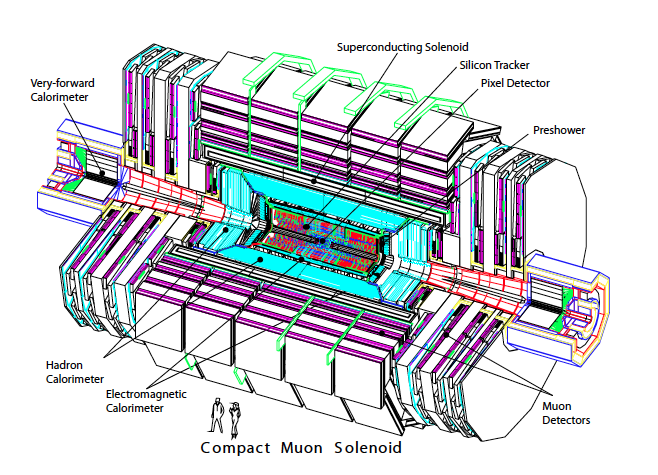
\includegraphics[width=1.0\columnwidth]{figures_chapter3/cms_detector}
\caption{A cutaway diagram of the CMS detector. The labels identify the different sub-detectors and the solenoid.}
\label{fig:cms}
\end{figure}

The CMS uses the right-handed coordinate system. The origin is centered at the nominal collision point, x-axis is in the horizontal plane pointing towards the centre of the LHC tunnel, y-axis points vertically upwards, and the z-axis points along the beam direction toward the Jura mountains. It is convenient to employ the spherical coordinate system. The polar angle  $\theta$ is measured with respect to the positive z-axis and the azimuthal angle $\theta$ is measured from the positive x-axis in the x-y coordinate plane. The pseudorapidity is defined as $\eta = -\ln \tan(\frac{\theta}{2})$.  A useful consequence of this definition is that the difference between the pseudorapidities of two particles is Lorentz invariant with respect to a boost in the beam direction. The separation of two particles is defined by $\Delta R = \sqrt(\Delta \phi^2 + \Delta \eta^2)$. The momentum and energy transverse to the beam direction are denoted $p_{T}$ and $E_{T}$ respectively. The imbalance of the measured transverse energy is defined as the missing energy and denoted by $E_{T}^{miss}$.     

\section{Inner tracking detectors}

The inner tracking system\cite{Karim�ki:368412,addendum} surrounds the interaction point and has a length of $5.8$ m and a diameter of $2.5$ m. The goal of the inner tracking system is to make a precise and efficient measurement of the trajectories of charged particles as well as their momentum. In addition a precise reconstruction of secondary vertices is needed for identification of heavy flavor particle decays. Tau lepton decays are identified by looking for one-prong and three-prong topologies in the inner tracker. A homogenous magnetic field of $4$ Tesla over the full volume of the tracker is provided by the CMS solenoid. 

There are $\Omega(1000)$ particles emerging from the interaction region at the nominal LHC luminosity for every $25$ ns bunch crossing. Therefore a high granular, fast, and radiation hard detector is required. On the other hand this implies a large power density of electronics and the corresponding cabling and cooling systems which increase the amount of material thereby enhancing multiple scattering, photon conversions, and bremsstrahlung.    Silicon technology was chosen given the above considerations. Figure~\ref{fig:tracker} shows a schematic view of the inner tracking system in $r-z$ plane. The inner tracking detector covers a pseudorapidity range of up to $\eta=2.5$ and provides an average $13-17$ measurements per charged particle depending on the $\eta$ region.

\begin{figure}[h]
\centering
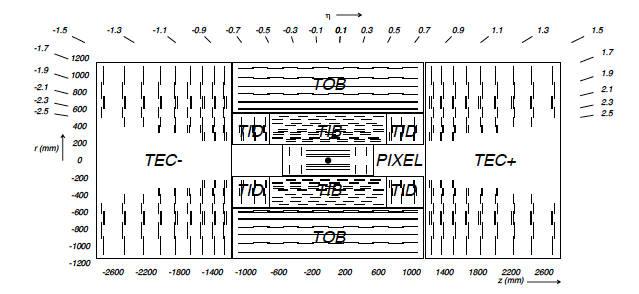
\includegraphics[width=1.0\columnwidth]{figures_chapter3/tracker_layout}
\caption{A schematic view of the CMS tracking system. Silicon pixel and strip detectors are shown. Double lines show back-to-back modules that deliver stereo hits.}
\label{fig:tracker}
\end{figure}

A pixelated detector has to be used close to the interaction region to keep the occupancy levels to less than $1\%$. It consists of three barrel layers and two endcap disks. The barrel layers are located at radii of $4.4$, $7.3$, and $10.2$ cm with a length of $53$ cm. The endcap pixel layers are located at $z=\pm 34.5$ and $z=\pm46.5$ cm covering approximately $6$ to $15$ cm in radial direction. The pixel detector consists of $66$ million pixel elements covering a surface area of approximately of $1$ m$^2$. The pixel element size is $100\times150$ $\mu$m$^2$ providing similar track resolution in both $r-\phi$ and $r-z$ directions. Each pixel is a $p-n$ semiconductor junction. When a charged particle passes through the depletion region of the junction an electron-hole pairs are created and subsequently collected by the readout electronics. The Lorentz drift in the CMS magnetic field leads to charge spreading of the collected signal charge between adjacent pixels. Using an analog pulse height read out the charge sharing allows to reduce a single hit spatial resolution to $15-20$ $\mu$m.  

The outer tracker is occupied by a silicon strip tracker allowing two-dimensional measurements. Majority of the strips are oriented perpendicular to the $\phi$ direction, parallel to the beam direction in the barrel region and aligned radially in the endcap region. The tracker Inner Barrel (TIB) is located in the barrel region and extends from $20$ cm to $55$ cm in the radial direction. There are $6$ additional layers with an outer radius of $116$ composing the Tracker Outer Barrel (TOB) and extending in $|z|$ to $118$ cm. The Tracker Disk (TID) consists of $3$ layers located from $|z|$ of $80$ and $90$ cm. The Tracker EndCap (TEC) has nine layers and covers the region between $|z|$ of  $124$ and $282$ cm. These radial strips provide up to  $9$ $\phi$ measurements for each trajectory. The silicon strip tracker has a total of $9.3$ million strips and covers a surface area of $198$ m$^2$. The strip pitch varies between $80$ and $184$ $\mu$m depending on the region of interest. In addition, there is a second strip module mounted back-to-back with a stereo angle of $100$ mrad in in the first layers. This allows a measurement of the $z$ and $r$ coordinates in the barrel and disks respectively. The corresponding resolution in z co-coordinate is $230$ to $530$ $\mu$m in TIB and TOB.  

\section{Electromagnetic calorimeter}

The goal of the CMS electromagnetic calorimeter (ECAL)\cite{ecal,CMS:2002xia} is to measure the energy of electrons and photons. ECAL is a homogeneous and hermetic calorimeter made of $61200$ lead tungstate (PbWO$_4$) crystals in the central barrel region (EB) and $14648$ crystals in the endcap region (EE). A homogeneous calorimeter was chosen to achieve the best energy resolution as one of the driving criteria was the precise measurement of the decay of the Higgs boson to two photons. Incident photons and electrons initiate an electromagnetic shower in the $PBWO_4$ crystals. The particles in the shower produce blue-green scintillation light as they excite the crystals and the scintillation light is measured by the photodetectors to determine the energy deposited in the crystals.   

Lead tungstate high density ($8.3$ g/cm$^3$) crystals were chosen to satisfy the challenging operational requirements at the LHC. The scintillation decay time of these crystals is of the same order as the LHC bunch crossing with $80\%$ of the light is emitted in $25$ ns. A short radiation length of $X_{0}=0.89$ cm and a small Moliere radius of $2.2$ cm allows to have a fine granular and a compact calorimeter while still containing the electromagnetic showers in longitudinal and transverse directions. The crystals are radiation hard but there is a transparency loss under exposure to an ionizing radiation with a dynamical recovery when there are no collisions. The transparency loss is corrected with a dedicated laser monitoring system. 

\begin{figure}[h]
\centering
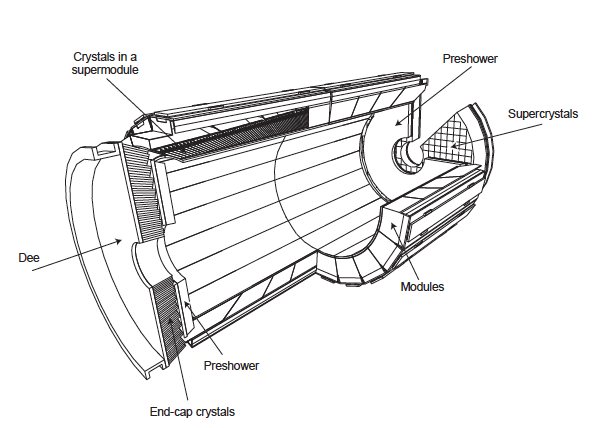
\includegraphics[width=1.0\columnwidth]{figures_chapter3/cms_ecal}
\caption{The layout of the CMS electromagnetic calorimeter. Barrel and endcap detectors are shown. The pre-shower detector sits in front of the endcap ecal.}
\label{fig:ecal}
\end{figure}

Figure\ref{fig:ecal} shows the layout of the ECAL. The $61200$ crystals in EB are arranged in a $170\times360$ $\eta-\phi$ grid with a coverage up to $|\eta|=1.479$ in presudorapidity. The crystal front face cross section is approximately $0.0174\times0.0174$ in $\eta-\phi$ ($22-22$ mm$^2$) and $26-26$ mm$^2$ at the rear face. The increase in cross sectional area of the rear face is consistent with the small Moliere radius allowing to contain the transverse development of the electromagnetic shower within few crystals with respect to the central crystal. Each crystal has a length of $230$ mm corresponding to $25.8$ radiation lengths allowing to contain the longitudinal shower development with negligible levels of leakage. The crystals make an angle of $3$ degrees with respect to the particle trajectories incident from the interaction vertex to avoid cracks alignment with the trajectories. Two avalanche photodiodes (APDs) with an active are of $5\times5$ mm$^2$ are connected to the back of the crystals to convert the scintillation light to photoelectrons.   

The $14648$ crystals in EE are arranged in an $x-y$ grid with a front face cross section of $28.62\times28.62$ mm$^2$ and a rear face cross section of $30\times30$ mm$^2$. The length of the crystals is $220$ mm corresponding to $24.7$ radiation lengths. Vacuum phototriodes (VPTs) with an active area of approximately  $280$ mm$^2$ allowing large surface coverage are used as photodetectors. An anode of very fine copper mesh allows to operate these devices in the $3.8$ Tesla magnetic field with only slight lose in gain. The EE extends the ECAL coverage from $|\eta|=1.479$ to $|\eta|=3.0$. A sampling preshower detector sits in front of the EE allowing the identification of neutral pions from $|\eta|=1.7$ to $|\eta|=2.6$. Two alternating layers of passive led and active silicon layers form a sampling calorimeter with approximately $3$ radiation lengths of the absorber material.  

The energy resolution of the ECAL can be parameterized as
\begin{equation} \label{eq:ecal_resol}
\frac{\sigma}{E} = \frac{S}{\sqrt{E}} \oplus  \frac{N}{E} \oplus C,
\end{equation}
where $E$ is the energy of the incident particle, $S$ is the stochastic term, $N$ is the noise term, and $C$ is the constant term. The longitudinal shower leakage is assumed to be negligible in (\ref{eq:ecal_resol}). Event-to-event fluctuations in the lateral shower containment and the photo-statistics of $2.1\%$ contribute to the stochastic term. The noise term is mostly due to the electronic and digitization noise while the constant term comes from intercalibration errors and a non-uniform light collection. Typical values found at an electron test beam are $S=0.029~\GeV^{\frac{1}{2}}$, $N=0.12~\GeV$, and $C=0.003$.    

\section{Hadronic calorimeter}

HCAL my friend.

\subsection{LS1 Upgrades}

\section{Muon Detectors}

\section{Triggering and Data Acquisition}
    



